% Created 2021-07-14 Wed 13:35
% Intended LaTeX compiler: pdflatex
\documentclass[presentation,mathserif,table]{beamer}
\usepackage[utf8]{inputenc}
\usepackage[T1]{fontenc}
\usepackage{graphicx}
\usepackage{grffile}
\usepackage{longtable}
\usepackage{wrapfig}
\usepackage{rotating}
\usepackage[normalem]{ulem}
\usepackage{amsmath}
\usepackage{textcomp}
\usepackage{amssymb}
\usepackage{capt-of}
\usepackage{hyperref}
\beamertemplatenavigationsymbolsempty
\usepackage[T1]{fontenc}
\usepackage{DejaVuSans}
\usefonttheme{professionalfonts}
\usepackage[euler-digits,euler-hat-accent]{eulervm}
\setbeamertemplate{itemize items}{•}
\setbeamertemplate{enumerate items}[default]
\setbeamertemplate{headline}{}
\setbeamertemplate{footline}{
\leavevmode%
\hbox{%
\begin{beamercolorbox}[wd=\paperwidth,ht=2.25ex,dp=1ex,right]{fg=black}%
\usebeamerfont{section in head/foot}\insertsection\hspace*{2em}
\insertframenumber{} / \inserttotalframenumber\hspace*{2ex}
\end{beamercolorbox}%
}%
\vskip0pt%
}
\usepackage{appendixnumberbeamer}
\setbeamersize{text margin left=3mm,text margin right=3mm}
\newcommand\blfootnote[1]{%
\begingroup
\renewcommand\thefootnote{}\footnote{#1}%
\addtocounter{footnote}{-1}%
\endgroup
}
\setbeamerfont{footnote}{size=\tiny}
\usepackage{tikz}
\usepackage[retainorgcmds]{IEEEtrantools}
\hypersetup{colorlinks=true, allcolors=., urlcolor=blue}
\usepackage[absolute,overlay]{textpos}
\newcommand{\eg}{e.g.\,}
\newcommand{\ie}{i.e.\,}
\newcommand{\aka}{a.k.a.\,}
\newcommand{\etc}{\emph{etc.}\,}
\newcommand{\X}{{\mathbold X}}
\newcommand{\bS}{{\mathbold S}}
\newcommand{\bSigma}{{\mathbold \Sigma}}
\newcommand{\x}{{\mathbold x}}
\newcommand{\bbeta}{{\mathbold \beta}}
\newcommand{\Y}{{\mathbold Y}}
\newcommand{\y}{{\mathbold y}}
\newcommand{\B}{{\mathbold B}}
\newcommand{\W}{{\mathbold W}}
\newcommand{\U}{{\mathbold U}}
\newcommand{\V}{{\mathbold V}}
\newcommand{\bH}{{\mathbold H}}
\newcommand{\R}{\mathbb{R}}
\DeclareMathOperator*{\argmin}{argmin}
\DeclareMathOperator*{\argmax}{argmax}
\DeclareMathOperator*{\tv}{TV}
\DeclareMathOperator*{\Tr}{Tr}
\DeclareMathOperator*{\FFT}{FFT}
\DeclareMathOperator*{\IFFT}{IFFT}
\DeclareMathOperator*{\diag}{diag}
\DeclareMathOperator*{\supp}{supp}
\DeclareMathOperator*{\tf}{tf}
\DeclareMathOperator*{\idf}{idf}
\DeclareMathOperator*{\df}{df}
\DeclareMathOperator*{\Var}{Var}
\DeclareMathOperator*{\Frob}{Frob}
\DeclareMathOperator*{\F}{F}
\DeclareMathOperator*{\softmax}{softmax}
\DeclareMathOperator*{\AUC}{AUC}
\usepackage{bm}
\usecolortheme{dove}
\setbeamercolor*{block title example}{fg=black,bg=white}
\setbeamercolor*{block body example}{fg=black,bg=white}
\usetheme{default}
\author{jerome dockes}
\date{}
\title{Machine learning Part 2}
\author{Jérôme Dockès \& Nikhil Bhagwat}
\titlegraphic{
\includegraphics[height=1.5cm]{figures/mcgill-university.png} \hspace{1.5cm} 
\includegraphics[height=1.5cm]{figures/origami-lab-logo.png}}
\date{QLS course 2021-07-30}
\subtitle{Dimensionality reduction \& cross-validation}
\hypersetup{
 pdfauthor={jerome dockes},
 pdftitle={Machine learning Part 2},
 pdfkeywords={},
 pdfsubject={},
 pdfcreator={Emacs 26.3 (Org mode 9.1.9)}, 
 pdflang={English}}
\begin{document}

\maketitle
\section{Intro}
\label{sec:org7bd1f5e}
\subsection{Recap of part 1}
\label{sec:org344bb4b}
\begin{frame}[label={sec:org9ee0135}]{Recap of part 1}
\begin{block}{Supervised learning}
\begin{itemize}
\item Regression: least-squares linear regression
\item Classification: logistic regression
\end{itemize}
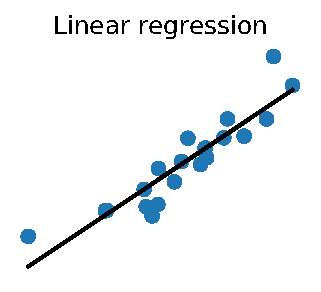
\includegraphics[height=.4 \textheight]{figures/generated/linear_regression_1d/linear_regression.pdf}
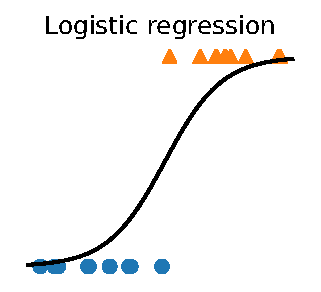
\includegraphics[height=.4 \textheight]{figures/generated/logistic_regression_1d/logistic_regression.pdf}
\end{block}
\end{frame}

\begin{frame}[label={sec:orgd22bf41}]{Recap of part 1}
\begin{block}<1->{Supervised learning}
\begin{itemize}
\item Regression: least-squares linear regression
\item Classification: logistic regression
\end{itemize}
\end{block}
\begin{block}<1->{Regularization}
\begin{itemize}
\item \(\ell_2\) \aka ridge regularization
\end{itemize}
\end{block}
\begin{block}<2->{Model evaluation and selection}
\begin{itemize}
\item Out-of-sample generalization; independent test set
\item Performance metrics:
\begin{itemize}
\item regression: mean squared error
\item classification: accuracy, ROC curve
\end{itemize}
\item Cross-validation
\end{itemize}
\end{block}
\begin{block}<3->{ }
Don't remember? watch Part 1 again!
\end{block}
\end{frame}
\begin{frame}[label={sec:orgda725f6}]{Notation \& vocabulary}
\begin{block}{Supervised learning framework}
\begin{equation}
Y = f(X) + E
\end{equation}
\vspace{-10pt}
\begin{itemize}[<+->]
\item \(Y \in \R\): output (\aka target, dependent variable) to predict
\item \(X \in \R^p\): features (\aka inputs, regressors, descriptors, independent variables)
\item \(E \in \R\): unmodelled noise
\item \(f\): the function we try to approximate
\end{itemize}
\end{block}
\begin{block}<4->{Example: linear regression}
\vspace{-20pt}
 \begin{IEEEeqnarray}{rCl}
 Y & = & \beta_0 + \langle X, \beta \rangle + E \\
& = & \beta_0 + \sum_{j=1}^p X_j \, \beta_j + E
 \end{IEEEeqnarray}
"learning" = estimating \(\beta_0 \in \R\) and \(\beta \in \R^p\)
\end{block}
\end{frame}
\begin{frame}[label={sec:org271027c}]{How to estimate parameters: Empirical Risk Minimization}
Given \(n\) training examples \(\X \in \R^{n \times p}\), \(\y \in \R^n\),

find \(\hat{\beta}_0 \in \R, \hat{\bbeta} \in \R^p\)

that minimize the empirical risk:
\begin{IEEEeqnarray}{rcl}
\| \y - \hat{\y} \|_2^2 & \; = \; & \| \y - \hat{\beta}_0 - \X \, \hat{\bbeta} \|_2^2 \\
& \; = \; & \sum_{i=1}^n (\y_i - \hat{\beta}_0 - \sum_{j=1}^p \X_{ij}\, \hat{\bbeta}_j )^2
\end{IEEEeqnarray}

"Fitting" the parameters to \(\X, \y\).
\end{frame}
\section{Dimensionality reduction}
\label{sec:orgabc8344}
\subsection{Intro}
\label{sec:org42b4af9}
\begin{frame}[label={sec:org671e794}]{Dimensionality reduction}
\begin{block}{Until now}
\begin{center}
\includegraphics[height=.12 \textheight]{figures/graphs/pipeline-1.pdf}
\end{center}
\end{block}
\begin{block}{Add a step in the pipeline: simplifying the inputs}
\begin{center}
\includegraphics[height=.12 \textheight]{figures/graphs/pipeline-2.pdf}
\end{center}
\end{block}
\end{frame}
\begin{frame}[label={sec:orgab2af43}]{Dimensionality reduction}
\begin{equation}
\hat{\y} = \hat{\beta}_0 + \hat{\bbeta}_1 \, \X_{:, 1} + \hat{\bbeta}_2 \, \X_{:, 1} + \dots + \hat{\bbeta}_p \, \X_{:, p}
\end{equation}
\begin{block}{Problems when the number of features \(p\) becomes large}
\begin{itemize}
\item Bigger errors on test data (larger variance of predictions)
\item Numerical stability issues
\item Computational cost and memory usage
\end{itemize}
\end{block}
\end{frame}
\begin{frame}[fragile,label={sec:org3597ff4}]{Simulated data for linear regression}
 \begin{itemize}
\item Generate \(\X \in \R^{n \times 3}\), \(\mathbold{\bbeta} \in \R^3\), \(\mathbold{e} \in \R^n\) and \(\y = \X \, \bbeta + \mathbold{e} \in R^n\)
\item Append columns containing random noise to \(\X\)
\item Now \(\X \in \R^{n \times p}\), with \(p \geq 3\), but only the first 3 columns are linked with \(\y\)
\item Split into training and testing tests and evaluate a linear regression model: what happens when \(p\) becomes large?
\end{itemize}

See \href{https://scikit-learn.org/stable/modules/generated/sklearn.datasets.make\_regression.html\#sklearn.datasets.make\_regression}{\texttt{sklearn.datasets.make\_regression}} for generating data
\begin{center}
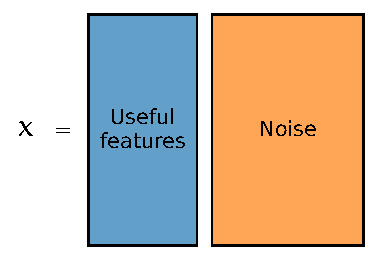
\includegraphics[height=.4 \textheight]{figures/generated/show_make_regression/x_construction.pdf}
\end{center}
\end{frame}
\begin{frame}[label={sec:orgd48d82d}]{Model complexity: overfitting}
\begin{itemize}
\item Model complexity increases with dimension.
\item Example: a linear model in dimension \(p\) can fit exactly (0 training error) any set of \(p + 1\) points.
\item Risk of overfitting: fitting exactly training data but failing on test data
\end{itemize}

\begin{center}
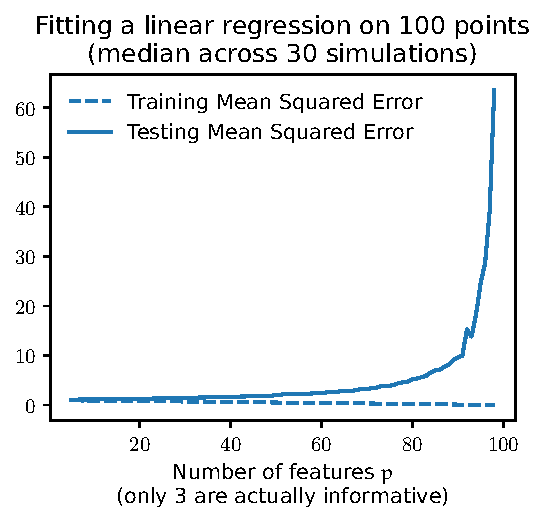
\includegraphics[height=.7\textheight]{figures/generated/ridge_overfitting/mse.pdf}
\end{center}
\end{frame}
\begin{frame}[label={sec:orge3a1435}]{Same plot in log scale}
\begin{center}
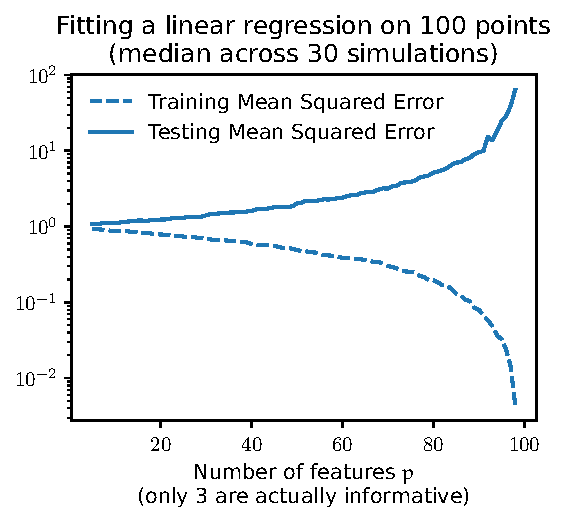
\includegraphics[height=.7\textheight]{figures/generated/ridge_overfitting/mse_log.pdf}
\end{center}
\end{frame}

\begin{frame}[label={sec:orgf0202d0}]{Cost of fitting many parameters}
\begin{itemize}
\item Many algorithms require polynomial time in \(p\)
\item Implementations often make copies of the design matrix (\eg for centering \& rescaling)
\end{itemize}
\begin{center}
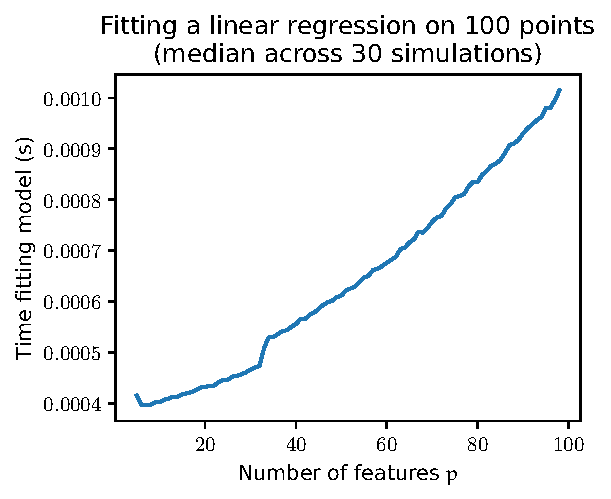
\includegraphics[height=.7\textheight]{figures/generated/ridge_overfitting/durations.pdf}
\end{center}
\end{frame}
\subsection{Univariate feature selection}
\label{sec:org3002ab8}
\begin{frame}[label={sec:org50f03c7}]{Solution 1: univariate feature selection}
\begin{itemize}
\item \aka feature screening, filtering \ldots{}
\item Check features (columns of \(\X\)) one by one for association with the output \(\y\)
\item Keep only a fixed number or percentage of the features
\end{itemize}
\begin{block}<2->{Simple (linear) association criteria}
\begin{itemize}
\item for regression: correlation
\item for classification: ANalysis Of VAriance
\end{itemize}
\end{block}
\begin{block}<2->{Read more in the scikit-learn user guide}
\url{https://scikit-learn.org/stable/modules/feature\_selection.html\#feature-selection}
\end{block}
\end{frame}

\begin{frame}[label={sec:orgec5a2b8}]{Simple selection criteria}
\begin{itemize}
\item Regression: correlation
\end{itemize}

\begin{center}
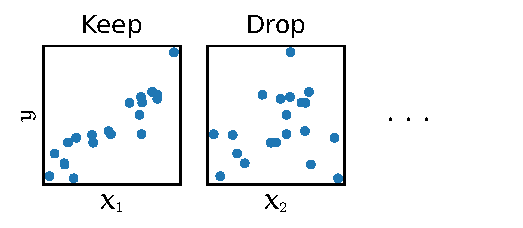
\includegraphics[height=.4 \textheight]{figures/generated/univariate_selection/regression.pdf}
\end{center}
\begin{itemize}
\item Classification: ANOVA
\end{itemize}
\vspace{-2pt}
\begin{center}
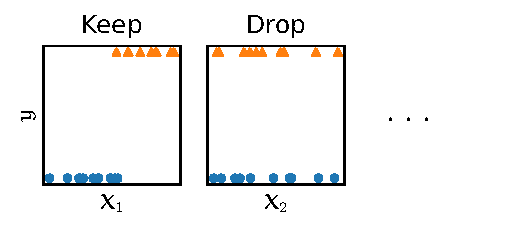
\includegraphics[height=.4 \textheight]{figures/generated/univariate_selection/classification.pdf}
\end{center}
\end{frame}

\begin{frame}[label={sec:org2a449b3}]{Univariate feature selection}
Keeping only the 10 best features (most correlated with \(\y\))
\begin{center}
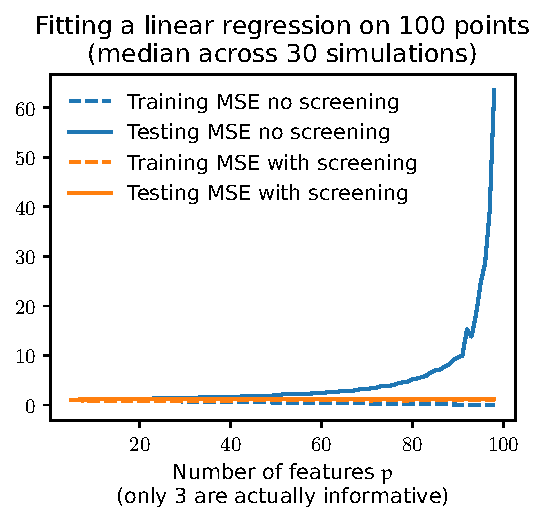
\includegraphics[height=.7\textheight]{figures/generated/ridge_overfitting/mse_with_dim_reduction.pdf}
\end{center}
\end{frame}

\begin{frame}[label={sec:org037f245}]{Same plot in log scale}
\begin{center}
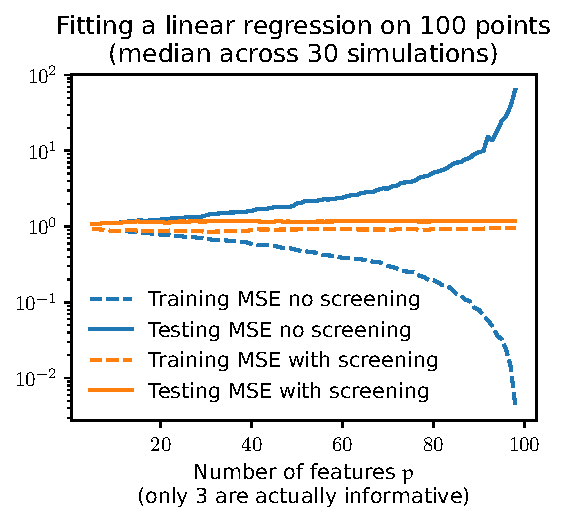
\includegraphics[height=.7\textheight]{figures/generated/ridge_overfitting/mse_with_dim_reduction_log.pdf}
\end{center}
\end{frame}

\subsection{Linear decomposition methods}
\label{sec:orgffcf913}
\begin{frame}[label={sec:org7d3988f}]{Solution 2: linear decomposition methods}
\begin{block}{Maybe OK to drop \(\X_2\):}
\vspace{-10pt}
\begin{center}
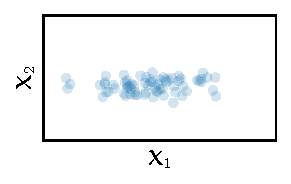
\includegraphics[height=.3\textheight]{figures/generated/pca/cloud_aligned.pdf}
\end{center}
\vspace{-20pt}
\end{block}
\begin{block}{Data low-dimensional but no feature can be dropped:}
\begin{center}
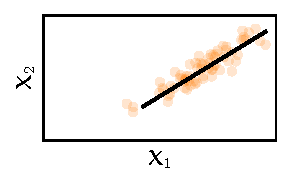
\includegraphics[height=.3\textheight]{figures/generated/pca/cloud_not_aligned.pdf}
\end{center}

Find a better referential in which to represent the data
\end{block}
\end{frame}
\begin{frame}[label={sec:org56b0d78}]{Linear regression: projection on the column space of \(X\)}
\begin{structureenv} %% top
\begin{columns}
\begin{column}{.3\columnwidth}
\begin{equation}
\hat{\y} = \X \, \hat{\bbeta}
\end{equation}
\end{column}

\begin{column}{.7\columnwidth}
\vspace{-17pt}
\begin{center}
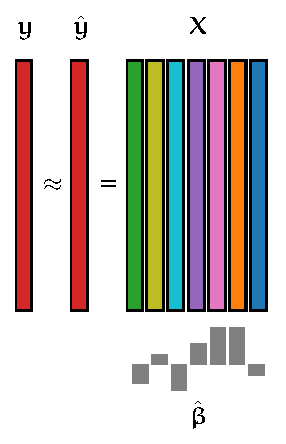
\includegraphics[height=.7\textheight]{figures/generated/dim_reduction_colors/regression_full_3.pdf}
\end{center}
\end{column}
\end{columns}
\end{structureenv}

\begin{structureenv} %% bottom
\begin{itemize}
\item Too many features: high variance \& unstable solution
\item Feature selection: drop some columns of \(\X\)
\item Other ways to build a family of \(k\) vectors on which to regress \(\y\)?
\end{itemize}
\end{structureenv}
\end{frame}
\begin{frame}[label={sec:org5972f8f}]{Linear decomposition: low-rank approximation of \(\X\)}
Minimize
\begin{equation}
\| \X - \W \, \bH \|_{\F}^2 = \sum_{i, j} ( \X_{i,j} - (\W \, \bH)_{i,j})^2
\end{equation}
\begin{center}
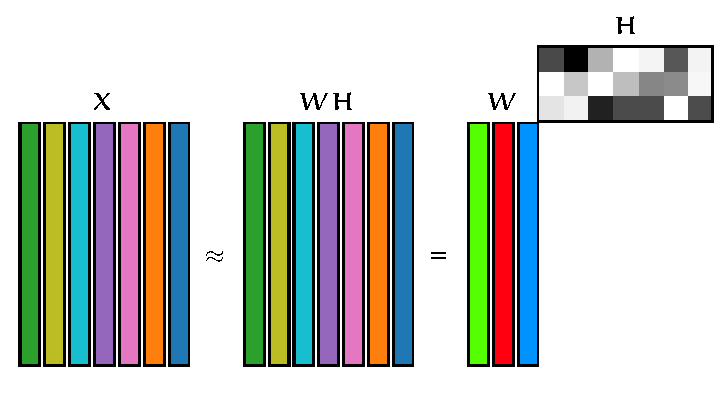
\includegraphics[height=.5\textheight]{figures/generated/dim_reduction_colors/factorization_3.pdf}
\end{center}
\end{frame}
\begin{frame}[label={sec:org0172df8}]{Linear regression after dimensionality reduction}
\begin{equation}
\hat{\y} = \W \, \hat{\bbeta}
\end{equation}
\begin{center}
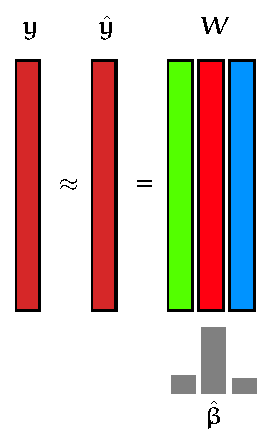
\includegraphics[height=.7\textheight]{figures/generated/dim_reduction_colors/regression_reduced_3.pdf}
\end{center}
\end{frame}
\begin{frame}[label={sec:org58533f8}]{Prediction for a new data point \(\x \in \R^{p}\)}
\begin{itemize}
\item Find the combination of rows of \(\bH\) that is closest to \(\x\): regress \(\x\) on \(\bH^T\)
\item Multiply by \(\hat{\bbeta}\)
\end{itemize}
    \begin{equation}
\x \in \R^p \rightarrow \text{projection} \rightarrow \mathbold{w} \in \R^k \rightarrow \langle \cdot \, , \, \hat{\bbeta}\rangle \rightarrow \hat{y} \in \R
    \end{equation}
\end{frame}
\begin{frame}[label={sec:orga0f6acf}]{Principal Component Analysis}
\begin{itemize}
\item Singular Value Decomposition of \(\X\):
\end{itemize}
\begin{equation}
\X = \U \, \bS \, \V^T
\end{equation}
with \(\X \in \R^{n \times p}\), \(\U \in \R^{n \times r}\), \(\bS \in \R^{r \times r}\), \(\V \in \R^{r \times p}\)
\begin{itemize}
\item \(r = \min(n, p)\)
\item \(\bS \succeq 0\) diagonal with decreasing values \(s_j\) along the diagonal
\item \(\U^T\, \U = I_r\)
\item \(\V^T\, \V = I_r\)
\end{itemize}

Truncating the SVD to keep only the first \(k\) components gives the best rank-\(k\) approximation of \(\X\)
\begin{center}
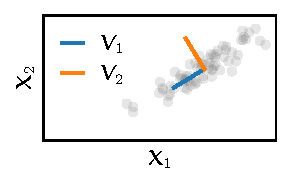
\includegraphics[height=.3\textheight]{figures/generated/pca/cloud_not_aligned_with_pc.pdf}
\end{center}
\end{frame}
\begin{frame}[label={sec:orgc0fecbf}]{Singular Value Decomposition}
\begin{equation}
\X = \U \, \bS \, \V^T
\end{equation}
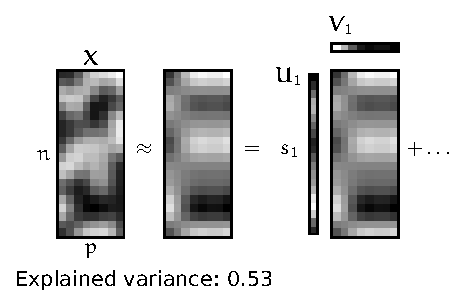
\includegraphics[height=.5 \textheight]{figures/generated/pca_step_by_step/pca_steps_1.pdf}

\begin{equation}
\U^T \, \U = I_p
\end{equation}
\begin{equation}
\V^T \, \V = I_p
\end{equation}
\end{frame}

\begin{frame}[label={sec:org9fd6c22}]{Singular Value Decomposition}
\begin{equation}
\X = \U \, \bS \, \V^T
\end{equation}
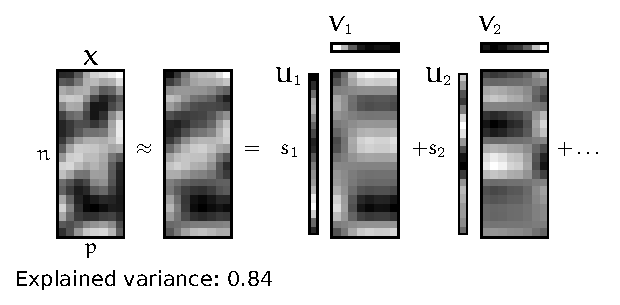
\includegraphics[height=.5 \textheight]{figures/generated/pca_step_by_step/pca_steps_2.pdf}

\begin{equation}
\U^T \, \U = I_p
\end{equation}
\begin{equation}
\V^T \, \V = I_p
\end{equation}
\end{frame}


\begin{frame}[label={sec:org10073cf}]{Singular Value Decomposition}
\begin{equation}
\X = \U \, \bS \, \V^T
\end{equation}
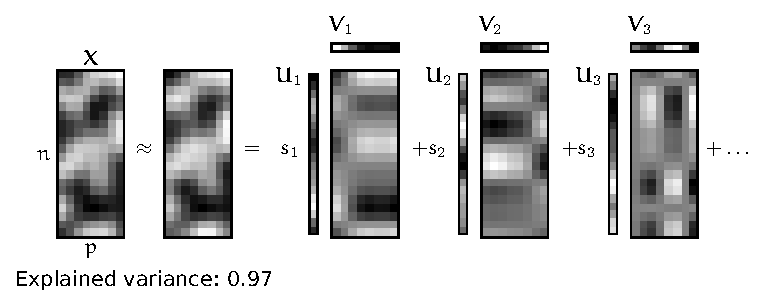
\includegraphics[height=.5 \textheight]{figures/generated/pca_step_by_step/pca_steps_3.pdf}

\begin{equation}
\U^T \, \U = I_p
\end{equation}
\begin{equation}
\V^T \, \V = I_p
\end{equation}
\end{frame}

\begin{frame}[label={sec:org5db5256}]{Other decomposition methods}
Many other methods use the same objective (sum of squared reconstruction errors), but add penalties or constraints on the factors
\begin{itemize}
\item Dictionary Learning
\item Non-negative Matrix Factorization
\item K-means clustering
\item \ldots{}
\end{itemize}

\begin{block}{What about \(\y\)?}
\begin{itemize}
\item PCA is an example of \emph{unsupervised} learning: it does not use \(\y\)
\item Some other methods take it into account: \eg Partial Least Squares
\end{itemize}
\end{block}
\end{frame}
\begin{frame}[label={sec:org02e9260}]{Ridge regression and PCA}
\begin{itemize}
\item Both ridge regression and PC regression compute the coordinates of \(\y\) in the basis given by the SVD of \(\X\)
\item Ridge shrinks the coordinate along \(\U_j\) by a factor \(s_j^2 / (s_j^2 + \lambda)\)
\item PC regression sets the coordinates to 0 except for those corresponding to the \(k\) largest \(s_j\): shrinks by a factor \(\mathbold{1}_{\{j \leq k\}}\)
\end{itemize}

\begin{center}
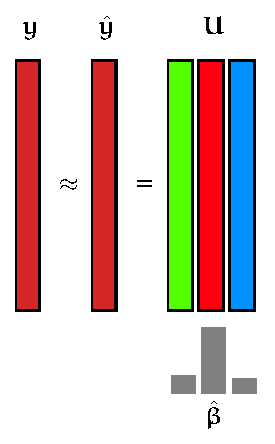
\includegraphics[height=.6\textheight]{figures/generated/dim_reduction_colors/regression_reduced_3_svd.pdf}
\end{center}
\end{frame}
\section{More on cross-validation}
\label{sec:org2e77a82}
\subsection{More on cross-validation}
\label{sec:orgc60166f}

\begin{frame}[label={sec:orgf0e54a7}]{Setting hyperparameters}
\begin{block}{How can we choose:}
\begin{itemize}
\item Number of features or PCA components \(k\)?
\item The ridge hyperparameter \(\lambda\)?
\end{itemize}
\end{block}
Try a few and pick the best one\ldots{}

But measure its performance on separate data!
\end{frame}
\begin{frame}[label={sec:org85c819b}]{Need for fresh test data}
When you hear "best", "maximum", "select", \ldots{} think "bias"
\begin{itemize}
\item I have 4 dice and want to find one that rolls high numbers
\item I roll them all once and select the die that gives the highest number
\item The selected die rolled a 5. Is 5 a good estimate of that die's average result? What if I had 1,000 dice?
\item I need to roll it again to get an unbiased estimate
\end{itemize}
\begin{center}
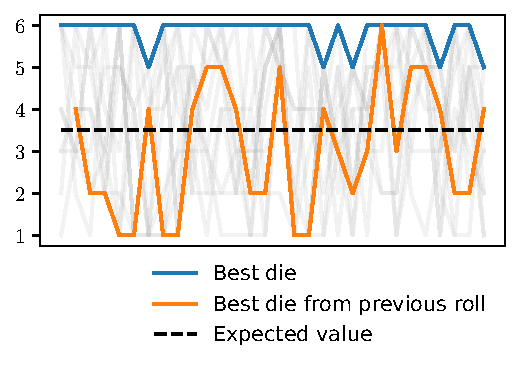
\includegraphics[height=.5 \textheight]{figures/generated/regression_to_mean/dice_rolls.pdf}
\end{center}
\end{frame}
\begin{frame}[label={sec:org1f85617}]{Nested cross-validation}
When you hear "best", "maximum", "select", \ldots{} think "bias"
\begin{block}<2->{Setting the parameters}
\begin{itemize}
\item \alert{Select} \(\bbeta\) that gives the \alert{best} prediction on training data
\item The prediction score for \(\hat{\bbeta}\) is biased: compute a new score on unseen test data.
\end{itemize}
\end{block}
\begin{block}<3->{Setting the hyperparameters}
\begin{itemize}
\item Repeat step 1 for a few values of \(\lambda\), \(k\), \etc., fitting and testing several models
\item \alert{Select} the hyperparameter that obtains the \alert{best} prediction on test data
\item The prediction score of that model on \emph{test} data is biased: evaluate it again on unseen data
\end{itemize}
\end{block}
\end{frame}
\begin{frame}[label={sec:orgd1f0f43}]{One split}
\begin{center}
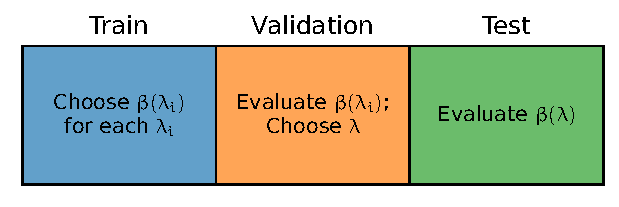
\includegraphics[width=.9\linewidth]{figures/generated/train_eval_test/datasets.pdf}
\end{center}
\end{frame}
\begin{frame}[fragile,label={sec:orgbef5ec8}]{Nested cross-validation}
 \begin{center}
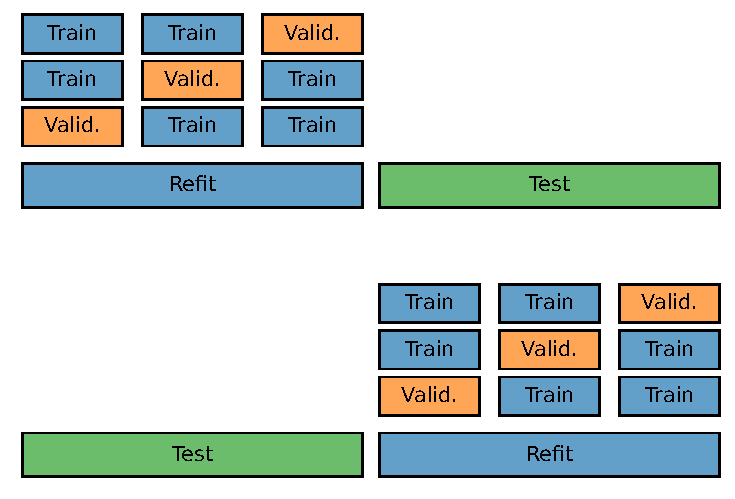
\includegraphics[width=.9\linewidth]{figures/generated/train_eval_test/cv.pdf}
\end{center}
see  \href{https://scikit-learn.org/stable/modules/generated/sklearn.model\_selection.GridSearchCV.html}{\texttt{sklearn.model\_selection.GridSearchCV}}
\end{frame}
\begin{frame}[fragile,label={sec:org491de6a}]{Some common pitfalls with cross-validation}
 \begin{block}<1->{Fitting part of the pipeline on the whole dataset}
\begin{itemize}
\item \eg fit PCA on all data, then do cross-validation on dim-reduced dataset
\item use  \href{https://scikit-learn.org/stable/modules/generated/sklearn.pipeline.Pipeline.html}{\texttt{sklearn.pipeline.Pipeline}}
\end{itemize}
\end{block}
\begin{block}<2->{Ignoring dependencies between samples}
\begin{itemize}
\item Multiple datapoints per participant
\item Time series
\end{itemize}
\end{block}
\begin{block}<3->{Ignoring dependencies between CV scores}
\begin{itemize}
\item Training sets overlap: cross-validation scores of different splits are not independent
\end{itemize}
\end{block}
\begin{block}<4->{Over-interpreting good CV scores}
\begin{itemize}
\item Good CV scores on one dataset do not mean the model will always perform well on a new dataset
\end{itemize}
\end{block}
\end{frame}

\begin{frame}[label={sec:org620676f}]{Split choice example: time series}
Which is easier?
\begin{center}
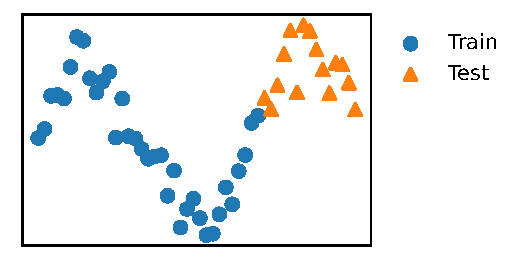
\includegraphics[height=.4 \textheight]{figures/generated/time_series_cv/kfold.pdf}
\end{center}

\begin{center}
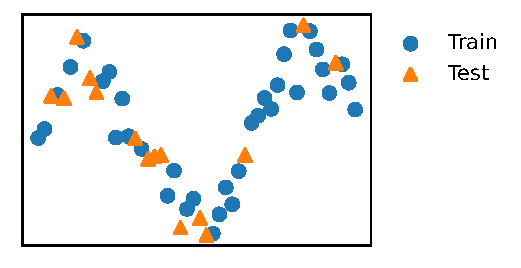
\includegraphics[height=.4 \textheight]{figures/generated/time_series_cv/kfold_shuffled.pdf}
\end{center}
\end{frame}
\begin{frame}[label={sec:orgeaba1c6}]{Remember that CV training sets overlap}
\begin{center}
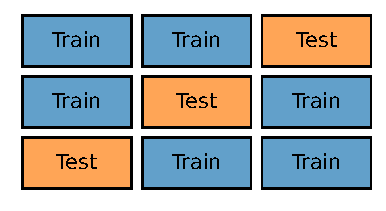
\includegraphics[height=.6 \textheight]{figures/generated/train_eval_test/cv_not_nested.pdf}
\end{center}

So the scores are not independent! Their variance can be underestimated.
\end{frame}
\section{Neuroimaging application: a task-fMRI prediction pipeline}
\label{sec:orgabf6775}
\subsection{FMRI decoding}
\label{sec:org74fce5e}
\begin{frame}[label={sec:org4a66dea}]{Supervised learning with fMRI}
\begin{itemize}
\item Predict in which site / with which scanner a resting-state fMRI sequence was acquired
\end{itemize}
\end{frame}
\begin{frame}[label={sec:org917adae}]{The prediction pipeline}
\begin{itemize}
\item Masking: extracting voxels that are inside the brain
\item Connectivity: measuring correlations between brain regions to build a feature vector for each participant
\item Univariate feature selection with ANalysis Of VAriance
\item Classifier: logistic regression
\end{itemize}
\end{frame}
\begin{frame}[label={sec:orgcc84cde}]{Implementation: in class}
\end{frame}
\end{document}
